\documentclass{beamer}
\usepackage{amsmath}
\usepackage[english]{babel} %set language; note: after changing this, you need to delete all auxiliary files to recompile
\usepackage[utf8]{inputenc} %define file encoding; latin1 is the other often used option
\usepackage{csquotes} % provides context sensitive quotation facilities
\usepackage{graphicx} %allows for inserting figures
\usepackage{booktabs} % for table formatting without vertical lines
\usepackage{textcomp} % allow for example using the Euro sign with \texteuro
\usepackage{stackengine}
\usepackage{wasysym}
\usepackage{tikzsymbols}
\usepackage{textcomp}
\newcommand{\bubblethis}[2]{
        \tikz[remember picture,baseline]{\node[anchor=base,inner sep=0,outer sep=0]%
        (#1) {\underline{#1}};\node[overlay,cloud callout,callout relative pointer={(0.2cm,-0.7cm)},%
        aspect=2.5,fill=yellow!90] at ($(#1.north)+(-0.5cm,1.6cm)$) {#2};}%
    }%
\tikzset{face/.style={shape=circle,minimum size=4ex,shading=radial,outer sep=0pt,
        inner color=white!50!yellow,outer color= yellow!70!orange}}
%% Some commands to make the code easier
\newcommand{\emoticon}[1][]{%
  \node[face,#1] (emoticon) {};
  %% The eyes are fixed.
  \draw[fill=white] (-1ex,0ex) ..controls (-0.5ex,0.2ex)and(0.5ex,0.2ex)..
        (1ex,0.0ex) ..controls ( 1.5ex,1.5ex)and( 0.2ex,1.7ex)..
        (0ex,0.4ex) ..controls (-0.2ex,1.7ex)and(-1.5ex,1.5ex)..
        (-1ex,0ex)--cycle;}
\newcommand{\pupils}{
  %% standard pupils
  \fill[shift={(0.5ex,0.5ex)},rotate=80] 
       (0,0) ellipse (0.3ex and 0.15ex);
  \fill[shift={(-0.5ex,0.5ex)},rotate=100] 
       (0,0) ellipse (0.3ex and 0.15ex);}

\newcommand{\emoticonname}[1]{
  \node[below=1ex of emoticon,font=\footnotesize,
        minimum width=4cm]{#1};}
\usepackage{scalerel}
\usetikzlibrary{positioning}
\usepackage{xcolor,amssymb}
\newcommand\dangersignb[1][2ex]{%
  \scaleto{\stackengine{0.3pt}{\scalebox{1.1}[.9]{%
  \color{red}$\blacktriangle$}}{\tiny\bfseries !}{O}{c}{F}{F}{L}}{#1}%
}
\newcommand\dangersignw[1][2ex]{%
  \scaleto{\stackengine{0.3pt}{\scalebox{1.1}[.9]{%
  \color{red}$\blacktriangle$}}{\color{white}\tiny\bfseries !}{O}{c}{F}{F}{L}}{#1}%
}
\usepackage{fontawesome} % Social Icons
\usepackage{epstopdf} % allow embedding eps-figures
\usepackage{tikz} % allows drawing figures
\usepackage{amsmath,amssymb,amsthm} %advanced math facilities
\usepackage{lmodern} %uses font that support italic and bold at the same time
\usepackage{tikz}
\usepackage{tcolorbox}

\usefonttheme[onlymath]{serif} %set math font to serif ones

\definecolor{beamerblue}{rgb}{0.2,0.2,0.7} %define beamerblue color for later use

%%% defines highlight command to set text blue
\newcommand{\highlight}[1]{{\color{blue}{#1}}}


%%%%%%% commands defining backup slides so that frame numbering is correct

\newcommand{\backupbegin}{
   \newcounter{framenumberappendix}
   \setcounter{framenumberappendix}{\value{framenumber}}
}
\newcommand{\backupend}{
   \addtocounter{framenumberappendix}{-\value{framenumber}}
   \addtocounter{framenumber}{\value{framenumberappendix}}
}

%%%% end of defining backup slides

%Specify figure caption, see also http://tex.stackexchange.com/questions/155738/caption-package-not-working-with-beamer
\setbeamertemplate{caption}{\insertcaption} %redefines caption to remove label "Figure".
%\setbeamerfont{caption}{size=\scriptsize,shape=\itshape,series=\bfseries} %sets figure  caption bold and italic and makes it smaller


\usetheme{Boadilla}

% --------------------
% Overall information
% --------------------
\title[Economía I]{Economía I \vspace{4mm}
\\ Magistral ¿28?: ¡Repaso Final!}
\date{}
\author[Riottini]{Riottini Franco}
\vspace{0.4cm}
\institute[]{Universidad de San Andrés} 


\begin{document}

\begin{frame}
\titlepage
\centering
Magistral 26


\includegraphics[scale=0.2]{../Figures/logoUDESA.jpg} 
\end{frame}

\begin{frame}{Repaso: Monopolio}
    \begin{itemize}
        \item Una unica empresa vende un bien o servicio sin sustitutos cercanos.
        \item La empresa enfrenta la curva de demanda del mercado.
        \item La regla de maximización es siempre la misma: $IMg=CMg$, solo que en competencia perfecta $IMg = P$ y acá $IMg \neq P$.
    \end{itemize}
    Consideremos el siguiente ejemplo:
    \begin{itemize}
        \item Un monopolista enfrenta la curva de demanda \( p = 120 - 2q \). Además, su curva de costo total es \( CT(q) = 20 + 5q + q^2 \), siendo su correspondiente curva de costo marginal \( CMg(q) = 5 + 2q \).

        \begin{enumerate}
            \item ¿Cuánto producirá el monopolista y a qué precio venderá este bien si desea maximizar su beneficio?
            \item ¿Cuál es el máximo beneficio que puede obtener?
            \item ¿Cuál sería la cantidad que ofrecería este monopolista si se comportara como una empresa perfectamente competitiva?
            \item ¿Cuál es el costo de eficiencia del monopolio? Grafique.
        \end{enumerate}
    \end{itemize}
\end{frame}

\begin{frame}{Repaso: Monopolio}

\end{frame}

\begin{frame}{Repaso: Impuestos}
    \small
    \begin{itemize}
        \item Los impuestos generan desplazamientos "ficticios" en las curvas.
        \item Hay diferencias \textbf{gráficas} dependiendo de si el impuesto se cobra a vendedores o a compradores.
        \item El impuesto genera una pérdida de eficiencia.
        \item La carga del impuesto es distinta de acuerdo a la elasticidad de cada curva.
    \end{itemize}

    Sean las curvas de oferta y de demanda de café: \( P = 3Q + 12 \) y \( P = 200 - Q \), respectivamente. Las cantidades se expresan en kg.

    \begin{enumerate}
        \item Encuentre el precio y la cantidad de equilibrio y grafique.
        \item El gobierno impone un impuesto de \$20 por cada kg. de café vendido. Encuentre el equilibrio y grafique la situación luego de la política. Asuma que el impuesto se le cobra al productor. Calcule la recaudación y el excedente del consumidor y del productor.
        \item Calcule la carga del impuesto que recae sobre los oferentes y la carga del impuesto que recae sobre los demandantes.
        \item ¿Podemos saber si la demanda es más elástica que la oferta en el punto de equilibrio? Justifique.
    \end{enumerate}
\end{frame}

\begin{frame}{Repaso: Impuestos}

\end{frame}


\begin{frame}{Repaso: Externalidades}
    
    \scriptsize

    \begin{itemize}
        \item Las externalidades generan diferencias entre el costo marginal social y el costo marginal privado
        \item Hay dos tipos de externalidades: positivas y negativas
        \item Y también estan aquellas que se generan en el consumo o en la producción (por lo general vamos a ver las de producción)
        \item El punto Pareto eficiente será donde $CMgS = IMg$ (interpretarlo en contexto!)
    \end{itemize}

    Una fábrica está situada al lado de un dormitorio para enfermeras que trabajan en turnos nocturnos. La fábrica produce 120 unidades de robots por día. El proceso de producción es ruidoso, y las enfermeras suelen quejarse de que no pueden dormir. El siguiente gráfico muestra el MPC (marginal private cost) y el MSC (marginal social cost) de la producción de robots:

    \begin{figure}[h!]
        \centering
        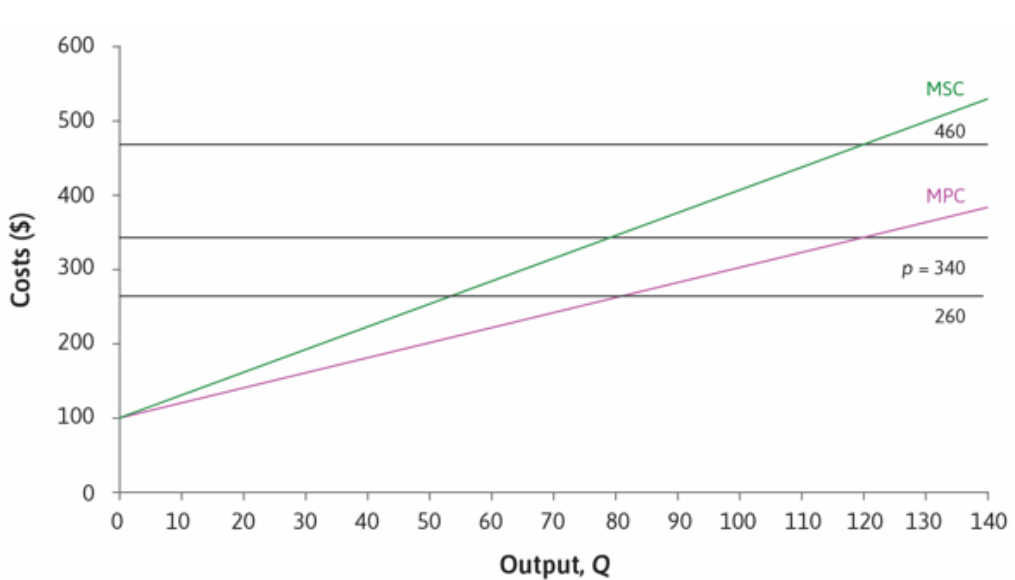
\includegraphics[width=0.6\textwidth]{../Figures/Externalidades_Ejercicio.png}
    \end{figure}

\end{frame}

\begin{frame}{Repaso: Externalidades}
    \scriptsize

    \begin{figure}[h!]
        \centering
        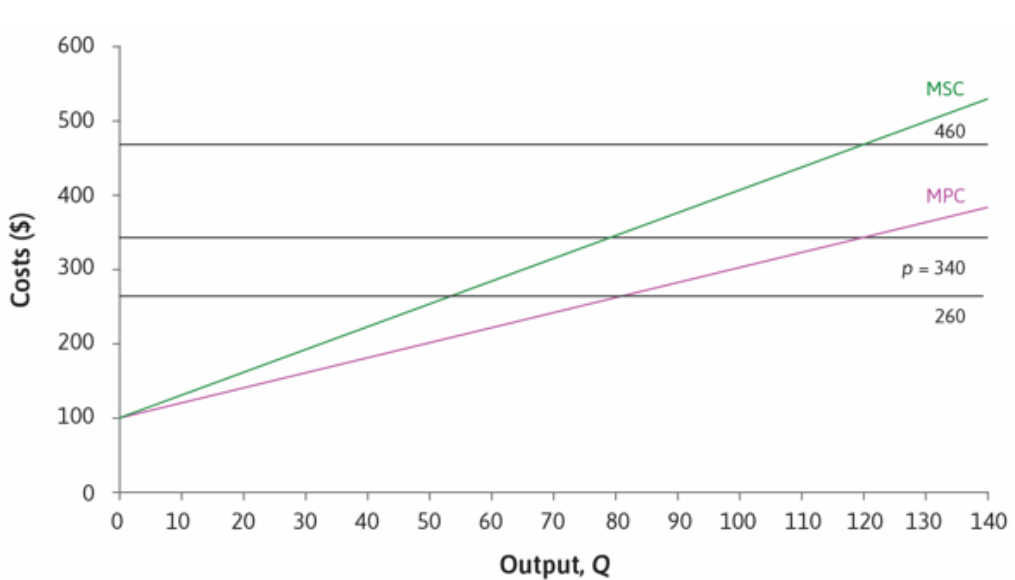
\includegraphics[width=0.5\textwidth]{../Figures/Externalidades_Ejercicio.png}
    \end{figure}

    El mercado de robots es competitivo y el precio de mercado es \$340. A partir de esta información, ¿cuál de las siguientes afirmaciones es correcta? Justifique sus respuestas.
    \begin{itemize}
        \item El nivel Pareto eficiente de producción es la cantidad maximizadora de beneficios de la fábrica: 120 unidades.
        \item El nivel Pareto eficiente de producción es cero, donde hay un costo marginal externo igual a cero para las enfermeras. 
        \item En \(Q = 120\), tanto la fábrica como las enfermeras se beneficiarían si las enfermeras pagaran una compensación de menos de \$120 a la fábrica por cada robot que dejen de producir.
        \item En \(Q = 80\), tanto la fábrica como las enfermeras se beneficiarían si la fábrica pagara una compensación de menos de \$80 a las enfermeras por cada robot adicional que produzcan.
    \end{itemize}

\end{frame}

\begin{frame}{Repaso: Mercado de trabajo}

    \begin{figure}[h!]
        \centering
        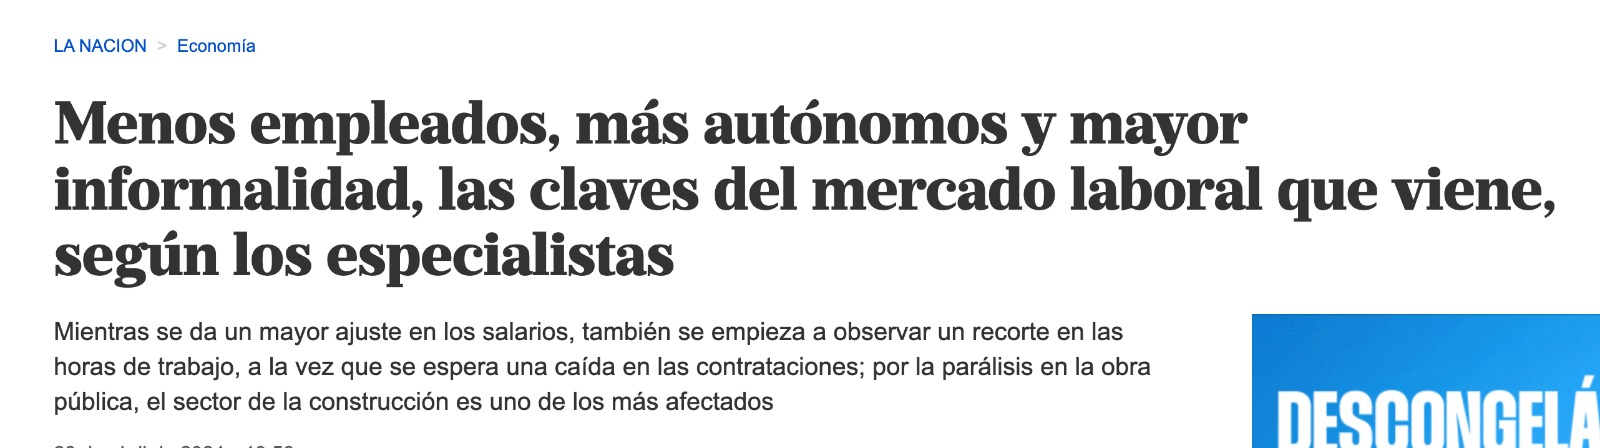
\includegraphics[width=1\textwidth]{../Figures/ejercicio_noticia0.jpg}
    \end{figure}

\end{frame}

\begin{frame}{Repaso: Mercado de trabajo}
    
\end{frame}

\begin{frame}{Repaso: Política Fiscal}
    La economía de Groenlandia experimenta un conflicto geopolítico en Oriente que provoca un abrupto aumento en el precio global del petróleo. Siendo Groenlandia un productor de petróleo, enfrenta costos de producción más altos, lo que repercute en casi todos los sectores de su economía.
    \begin{enumerate}
        \item Dado este contexto, ¿cómo se ajustarán los precios y el producto y por qué? Responda y grafique desde la perspectiva clásica y keynesiana.
        \item ¿Qué herramientas de política económica recomendaría cada escuela de pensamiento para abordar estos shocks y por qué?
        \item Suponga que el Banco Central está pensando en comprar dólares y quiere conocer cuáles serán los efectos en equilibrio general de esta política monetaria. Muestre mediante un gráfico y explique qué pasará en el mercado de dinero y de bienes desde la perspectiva keynesiana. 
    \end{enumerate}
\end{frame}

\begin{frame}{Repaso: Política Fiscal}
    
\end{frame}

\begin{frame}{Repaso: Mecano 1}

    \begin{figure}[h!]
        \centering
        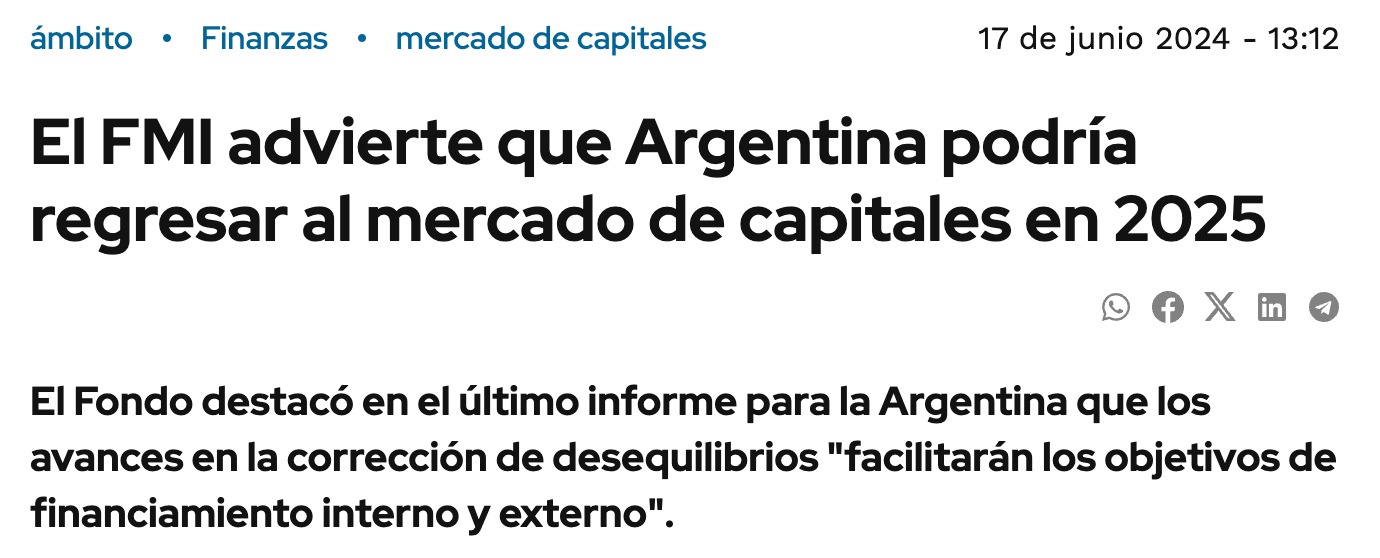
\includegraphics[width=1\textwidth]{../Figures/ejercicio_noticia1.jpg}
    \end{figure}
    ¿Cómo crees que esta noticia puede afectar a la inflación? ¿Por qué?
\end{frame}

\begin{frame}{Repaso: Mecano 1}
    
\end{frame}

\begin{frame}{Repaso: Mecano 2}

    \begin{figure}[h!]
        \centering
        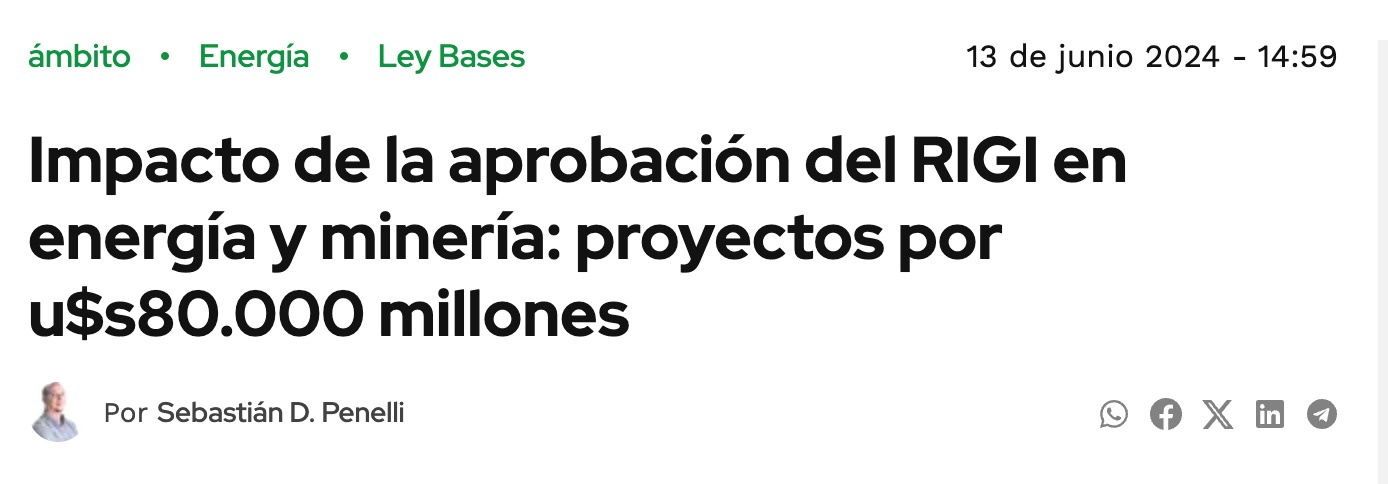
\includegraphics[width=1\textwidth]{../Figures/ejercicio_noticia2.jpg}
    \end{figure}
    Explique las consecuencias sobre el producto y la inflación de esta noticia bajo un mundo keynesiano y bajo un mundo clasico.
\end{frame}

\begin{frame}{Repaso: Mecano 2}
    
\end{frame}

\begin{frame}{Repaso: Mecano 3}

    \begin{figure}[h!]
        \centering
        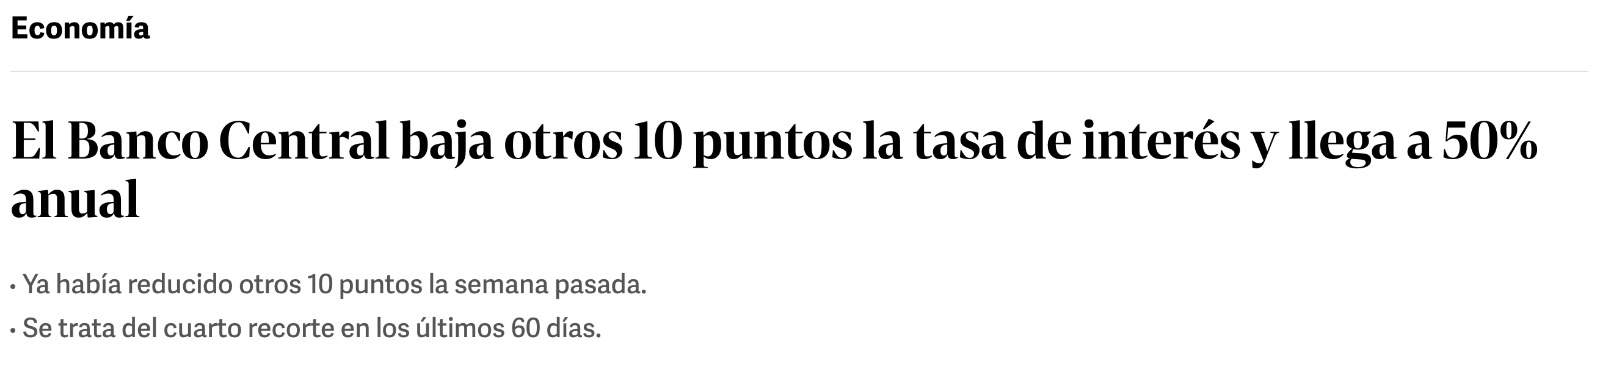
\includegraphics[width=1\textwidth]{../Figures/ejercicio_noticia3.jpg}
    \end{figure}
    ¿Que está sucediendo con la oferta de dinero dada esta noticia? ¿Como afecta al mercado monetario?¿Afecta al mercado de bienes? ¿Se tienen que dar algunas condiciones en particular para que esto último suceda?
\end{frame}

\begin{frame}{Repaso: Mecano 3}
    
\end{frame}

\end{document}







